%%!TeX program = xelatex
%% 부득이하게 pdflatex을 사용해야 할 경우 위의 magic comment를 제거하십시오.

% Initiated by 정민석(2014년도 경기과학고 수학과전문교원)
% Continously being modified by 경기과학고 TeX 사용자협회
% Website : http://gshslatexintro.github.io 

\documentclass{gshs_report}
% 아래의 함수를 사용하면 이미지 파일들을 같은 디렉토리 내에 images 라는 이름을 가진 폴더를 생성한 후, 그 폴더 안에 넣어 사용할 수 있습니다.
% 사용하고자 한다면 주석을 푸십시오.
\graphicspath{{images/}}
% 이곳에 필요한 별도의 패키지들을 적어넣으시오.
%\usepackage{...}
\usepackage{verbatim} % for commment, verbatim environment
\usepackage{spverbatim} % automatic linebreak verbatim environment
%\usepacakge{indentfirst}
\usepackage{tikz}
%\tikzset{
%	image label/.style={
%		every node/.style={
			%fill=black,
			%text=white,
%			font=\sffamily\scriptsize,
%			anchor=south west,
%			xshift=0,
%			yshift=0,
%			at={(0,0)}
%		}
%	}
%}
\usepackage{amsmath}
\usepackage{amsfonts}
\usepackage{amssymb}
\usepackage{float}
\usepackage{graphicx}
\usepackage{tabularx}
\usepackage{multirow}
\usepackage{booktabs}
\usepackage{longtable}
\usepackage{gensymb}
\usepackage{wrapfig}
%\usepackage{subcaption}
%\usepackage{floatrow}
%\usepackage{pict2e}
%\usepackage[backend=biber,style=authoryear]{biblatex}
%\usepackage{biblatex}
\usepackage{pgfplots}
\pgfplotsset{
	compat=newest,
	label style={font=\sffamily\scriptsize},
	ticklabel style={font=\sffamily\scriptsize},
	legend style={font=\sffamily\tiny},
	major tick length=0.1cm,
	minor tick length=0.05cm,
	every x tick/.style={black},
}

\usetikzlibrary{shapes}
\usetikzlibrary{plotmarks}
\usepackage{listings}
\usepackage{hologo}
\usepackage{makecell}

\lstset{
	basicstyle=\small\ttfamily,
	columns=flexible,
	breaklines=true
}

\citation
\bibdata

%: ----------------------------------------------------------------------
%:               보고서 정보를 입력하시오
% ----------------------------------------------------------------------
% 아래와 같은 command를 만들면 길이가 긴 용어를 간편하게 사용할 수 있습니다. 단, 이미 지정된 함수명들은 새로운 함수명으로 사용할 수 없습니다.
\newcommand{\gshs}{Gyeonggi Science High School for the Gifted }

\researchtype{기초} % 기초 / 심화
\reporttype{결과} % 중간 / 결과

\title{제목} % 제목 개행 시 \linebreak 사용. \\나 \newline 은 안됨.
\englishtitle{English title}% 제목 개행 시 \linebreak 사용. \\나 \newline 은 안됨.

\author[1] {} % 제 1 저자명
\email[1]{} % 제 1 저자 이메일
\author[2] {} % 제 2 저자명
\email[2]{} % 제 2 저자 이메일
\advisor{} % 지도교사명
\advisorEmail{} % 지도교사 이메일

%%%%%%%%%%%%%%%%%%%%%%%%%%%%%%%%%%%%%%%%%%%%%%%
%%%% researchtype이 '심화'일 경우에만 나타남 %%%%
\professor{} % 지도교수명
\professorEmail{professor@e-mail.address} % 지도교수 이메일
%%%%%%%%%%%%%%%%%%%%%%%%%%%%%%%%%%%%%%%%%%%%%%%%
\summitdate{}{}{} % 제출일 (연, 월, 일)
\newtheorem{definition}{정의}
 % usepackage 등의 명령어는 여기에.
\usepackage{cite}
\usepackage{textcomp}
\usepackage{tocloft}
\setlength{\cftbeforesecskip}{0pt}
\setlength{\cftbeforesubsecskip}{0pt}
\setlength{\cftbeforesubsubsecskip}{0pt}

% 본문 시작
\begin{document}

	%표지만들기
	%makecover 함수와 관련하여 "Underfull \hbox (badness 10000) in paragraph" 오류는 무시하십시오. (TeXstudio ver 2.9.4 오류 기준)
	%\makecover
	

	%\baselineskip=2.2em         % line spacing in the paragraph
	%\maketitle  % command to print the title page with above variables
\makecover  % command to print the title page with above variables

\setcounter{page}{1}
\renewcommand{\thepage}{\roman{page}}

%----------------------------------------------
%   Table of Contents (자동 작성됨)
%----------------------------------------------
\cleardoublepage
\addcontentsline{toc}{section}{Contents}
\setcounter{secnumdepth}{3} % organisational level that receives a numbers
\setcounter{tocdepth}{3}    % print table of contents for level 3
\baselineskip=2.2em
\tableofcontents


%----------------------------------------------
%     List of Figures/Tables (자동 작성됨)
%----------------------------------------------
\cleardoublepage
\clearpage
\listoffigures	% 그림 목록과 캡션을 출력한다. 만약 논문에 그림이 없다면 이 줄의 맨 앞에 %기호를 넣어서 코멘트 처리한다.

\cleardoublepage
\clearpage
\listoftables  % 표 목록과 캡션을 출력한다. 만약 논문에 표가 없다면 이 줄의 맨 앞에 %기호를 넣어서 코멘트 처리한다.


\cleardoublepage
\clearpage

%---------------------------------------------------------------------
%                  영문 초록을 입력하시오
%---------------------------------------------------------------------
%\begin{abstracts}     %this creates the heading for the abstract page
%	\addcontentsline{toc}{section}{Abstract}  %%% TOC에 표시
%	\noindent{
%			Put your abstract here. Once upon a time, \gshs said : `The first, and the best.'
%	}
%\end{abstracts}

%\cleardoublepage
%\clearpage

\begin{abstractskor}
	\addcontentsline{toc}{section}{초록}  %%% TOC에 표시
	\noindent{
현재 경기과학고에는 자동으로 다양한 기상 정보를 수집하는 자동기상관측장비(AWS)가 존재한다. 그러나 기존의 자동기상관측장비는 그 가격이 비싸고 학생들이 관측 결과에 접근하기 어렵다는 문제가 있었다. 따라서 본 연구에서는 비교적 가격이 저렴한 라즈베리파이(Raspberry Pi)에 각종 센서를 이용하고 센서가 수집한 정보를 Python과 C언어를 통해 정리하여 자동기상관측장비를 제작하였다. 또한 측정한 정보를 라즈베리파이 내부 저장소에 저장하고 이를 MariaDB의 데이터베이스에 전송 후 저장해 장시간 수집한 데이터를 체계적으로 관리할 수 있도록 하였으며, 추후 센서를 보정하고 수집한 기상 정보를 학교 웹사이트로 전송하여 학생들이 기상 정보를 쉽게 파악할 수 있도록 활용할 수 있을 것이다.
	}
\end{abstractskor}






 % Abstract
	
	%%%%%%%%%%%%%%%%%%%%%%%%%%%%%%%%%%%%%%%%%%%%%%%%%%%%%%%%%%%
	%%%% Main Document %%%%%%%%%%%%%%%%%%%%%%%%%%%%%%%%%%%%%%%%
	%%%%%%%%%%%%%%%%%%%%%%%%%%%%%%%%%%%%%%%%%%%%%%%%%%%%%%%%%%%
	\cleardoublepage
	\clearpage
	\renewcommand{\thepage}{\arabic{page}}
	\setcounter{page}{1}
	
	%각 장을 아래와 같이 sub 폴더 안에 만들어서 넣으면 편리하다.
	\section{서론}

\subsection{연구의 필요성}

현재 경기과학고등학교에는 자동으로 기상 상황을 관측하는 자동기상관측장비(AWS, Automatic Weather Station)가 하나 존재한다. 그러나 그 가격이 매우 비싸고 AWS의 유지보수가 어려우며 일반 학생들이 수집한 자료에 쉽게 접근하지 못한다는 단점이 존재한다. 또한 온도, 습도, 강우 여부 등의 기본적인 기상 정보는 우리의 일상생활에도 큰 영향을 미치기에 자신이 위치한 지역의 기상 상황을 정확히 필요하는 것이 중요하다. 기상청에서 동네예보를 하고 있으나,  국지적인 기상 상황을 파악하기에는 부족한 점이 존재한다. 그렇기에 학생들이 경기과학고등학교가 위치한 수원시 장안구 송죽동의 기상 상황을 쉽게 확인할 수 있도록 하는 것이 필요하다고 생각되어 본 연구를 진행하게 되었다.

\subsection{연구의 목적}
본 연구에서는 기존의 AWS 장치가 가지고 있던 단점을 보완하는 것을 목적으로 하였다. 최덕환, 임효혁, 김나영 (2016)의 연구에서는 Mems 센서를 활용하여 소형 AWS를 제작하였으나, 현재까지 라즈베리파이(Raspberry pi)를 사용하여 제작한 자동기상관측장비에 관한 연구는 진행되어 있지 않다.\cite{Ref1} 상대적으로 값이 저렴하고 프로그램의 수정이 쉬운 초소형 컴퓨터 기판인 라즈베리파이와 각종 센서들로 제작하여 AWS의 유지 및 보수를 쉽게 할 수 있도록 하였으며, 수집한 데이터는 라즈베리파이의 내부 저장소에 파일로 저장하고, 동시에 MariaDB 서버 데이터베이스에 전송하였다. 또한 본 연구에서 제작한 AWS 장비를 사용함로써 경기과학고등학교의 기상 상황을 실시간으로 쉽게 확인할 수 있을 것으로 기대된다. % body1
	\section{이론적 배경}

\subsection{제목}

내용
 % 이론적 배경
	\section{연구 과정}

\subsection{라즈베리파이에 운영체제 설치 및 네트워크 설치}
\subsubsection{Raspbian 운영체제 설치 및 기본 설정}
인터넷을 통해 라즈베리 파이의 OS인 Raspbain(라즈비안) 4.19, 라즈베리파이를 외부 컴퓨터에서 원격으로 접속하기 위한 VNC Viewer, 마이크로 SD 카드에 운영 체제를 전달하기 위한 balena Etcher v1.5.56을 내려받았다. balena Etcher를 사용해 라즈비안 파일을 마이크로 SD로 전송하고, SD카드는 라즈베리 파이에 삽입하여 라즈베리파이를 구동하였다. 라즈베리파이 2개에 OS를 설치하였으나 실제 센서 연결 및 프로그래밍은 하나의 라즈베리파이에서만 하였다.
구동 후 라즈베리파이에 HDMI선을 이용하여 모니터와 연결한 후 기본 설정을 하였다. 라즈베리파이 장비의 이름은 각각 AWS-01과 AWS-02, 외부 접속 비밀번호는 ‘경기과학고’로 하였다. Raspberry pi 3의 경우 WiFi 지역 설정을 한국으로 하면 접속이 되지 않는 오류가 있어 부득이하게 지역을 영국으로 하되 시간은 서울의 표준 시각(KST)을 사용하였다. 라즈베리파이에 GSHSPhysics01 공유기를 연결한 후 라즈베리파이의 내부 IP 주소가 각각 192.168.0.6과 192.168.0.4임을 확인해 노트북의 VNC Viewer를 사용하여 원격 접속하였다. VNC Viewer의 사용을 위해서는 라즈베리 파이 설정에서 VNC를 허용해야 한다.
\subsubsection{네트워크 및 공유기 설정}
라즈베리파이에서 수집한 정보를 서버로 전송하고 개인 노트북으로 라즈베리파이에 접속해 명령어 작업을 하기 위하여 라즈베리파이를 Wi-Fi 공유기 ‘GSHS-AWS01’에 새로 연결시켰다. 공유기의 IP는 192.168.0.1이다. 그 후 공유기의 DHCP 설정 페이지에서 라즈베리파이의 내부 IP 주소를 AWS-01은 192.168.0.101, AWS-02는 192.168.0.102로 고정시켰다. 라즈베리파이의 네트워크 설정(Network Prefernces)에서도 IPv4 주소를 AWS-02 기준으로 192.168.0.102, 라우터 주소를 192.168.0.1, DNS 주소를 168.126.63.1로 설정하였다. 라즈베리파이에 모니터를 연결하지 않고도 외부 컴퓨터에서 작업을 하기 위해서는 컴퓨터에 VNC Viewer를 설치 후 라즈베리파이에 연결해야 한다. 컴퓨터의 네트워크를 GSHS-AWS01에 연결 후 VNC Viewer에서 라즈베리파이에 접속하기 위해 라즈베리파이의 내부 IP 주소인 192.168.0.102를 입력한다. 그 후 사용자 이름에 pi, 비밀번호에 경기과학고를 입력했을 때 정상적으로 접속이 됨을 확인하였다.

\subsection{센서의 연결}

% Please add the following required packages to your document preamble:
% \usepackage{graphicx}
\begin{table}[]
	\caption{연구에서 사용한 센서의 목록}
	\label{SENSOR}
	\resizebox{\textwidth}{!}{%
		\begin{tabular}{|c|c|c|c|c|}
			\hline
			측정 자료 & 센서 이름     & 동작 전압          & 핀 사용량                    & 비고                    \\ \hline
			온습도   & dht22     & 3.3V           & 3                        & 10kΩ 저항 사용            \\ \hline
			기압    & BMP180    & 3.3V           & 6 (SPI 사용시), 4 (I2C 사용시) &                       \\ \hline
			미세먼지  & PMS7003   & 5V             & -                        & UART 통신 사용, USB 포트 사용 \\ \hline
			풍향    & DM2014    & 12$\sim$24V DC & -                        & ADC 사용                \\ \hline
			풍속    & SEN0170   & 7$\sim$24V DC  & -                        & ADC 사용                \\ \hline
			강우량   & p/n 80422 & 5V             & 2                        &                       \\ \hline
			ADC   & MCP3208   & V              & 6                        & 풍향, 풍속센서의 연결 위해 필요    \\ \hline
		\end{tabular}%
	}
\end{table}

\subsubsection{온습도 센서(DHT22)}
DHT22는 센서가 위치한 지역의 온도와 습도를 측정해주는 센서이다. DHT22는 3.3V의 입력 전압을 요구하므로 아래 회로도와 같이 전선을 연결한다. DHT22 센서의 연결을 위해서는 10kΩ 저항 1개, 3.3V 전압 핀 1개, GND 핀 1개, GPIO 핀 1개가 필요하다. 전선 연결 후 측정한 온도와 습도를 출력하기 위해 Python 명령어를 실행해 출력한다. 이때 온습도 센서가 값을 받아들여 출력하기 위해서는 파이썬 라이브러리가 필요하므로 Adafruit Python DHT 라이브러리를 다운로드받아 사용한다.

\begin{figure}[htbp]
	\centering
	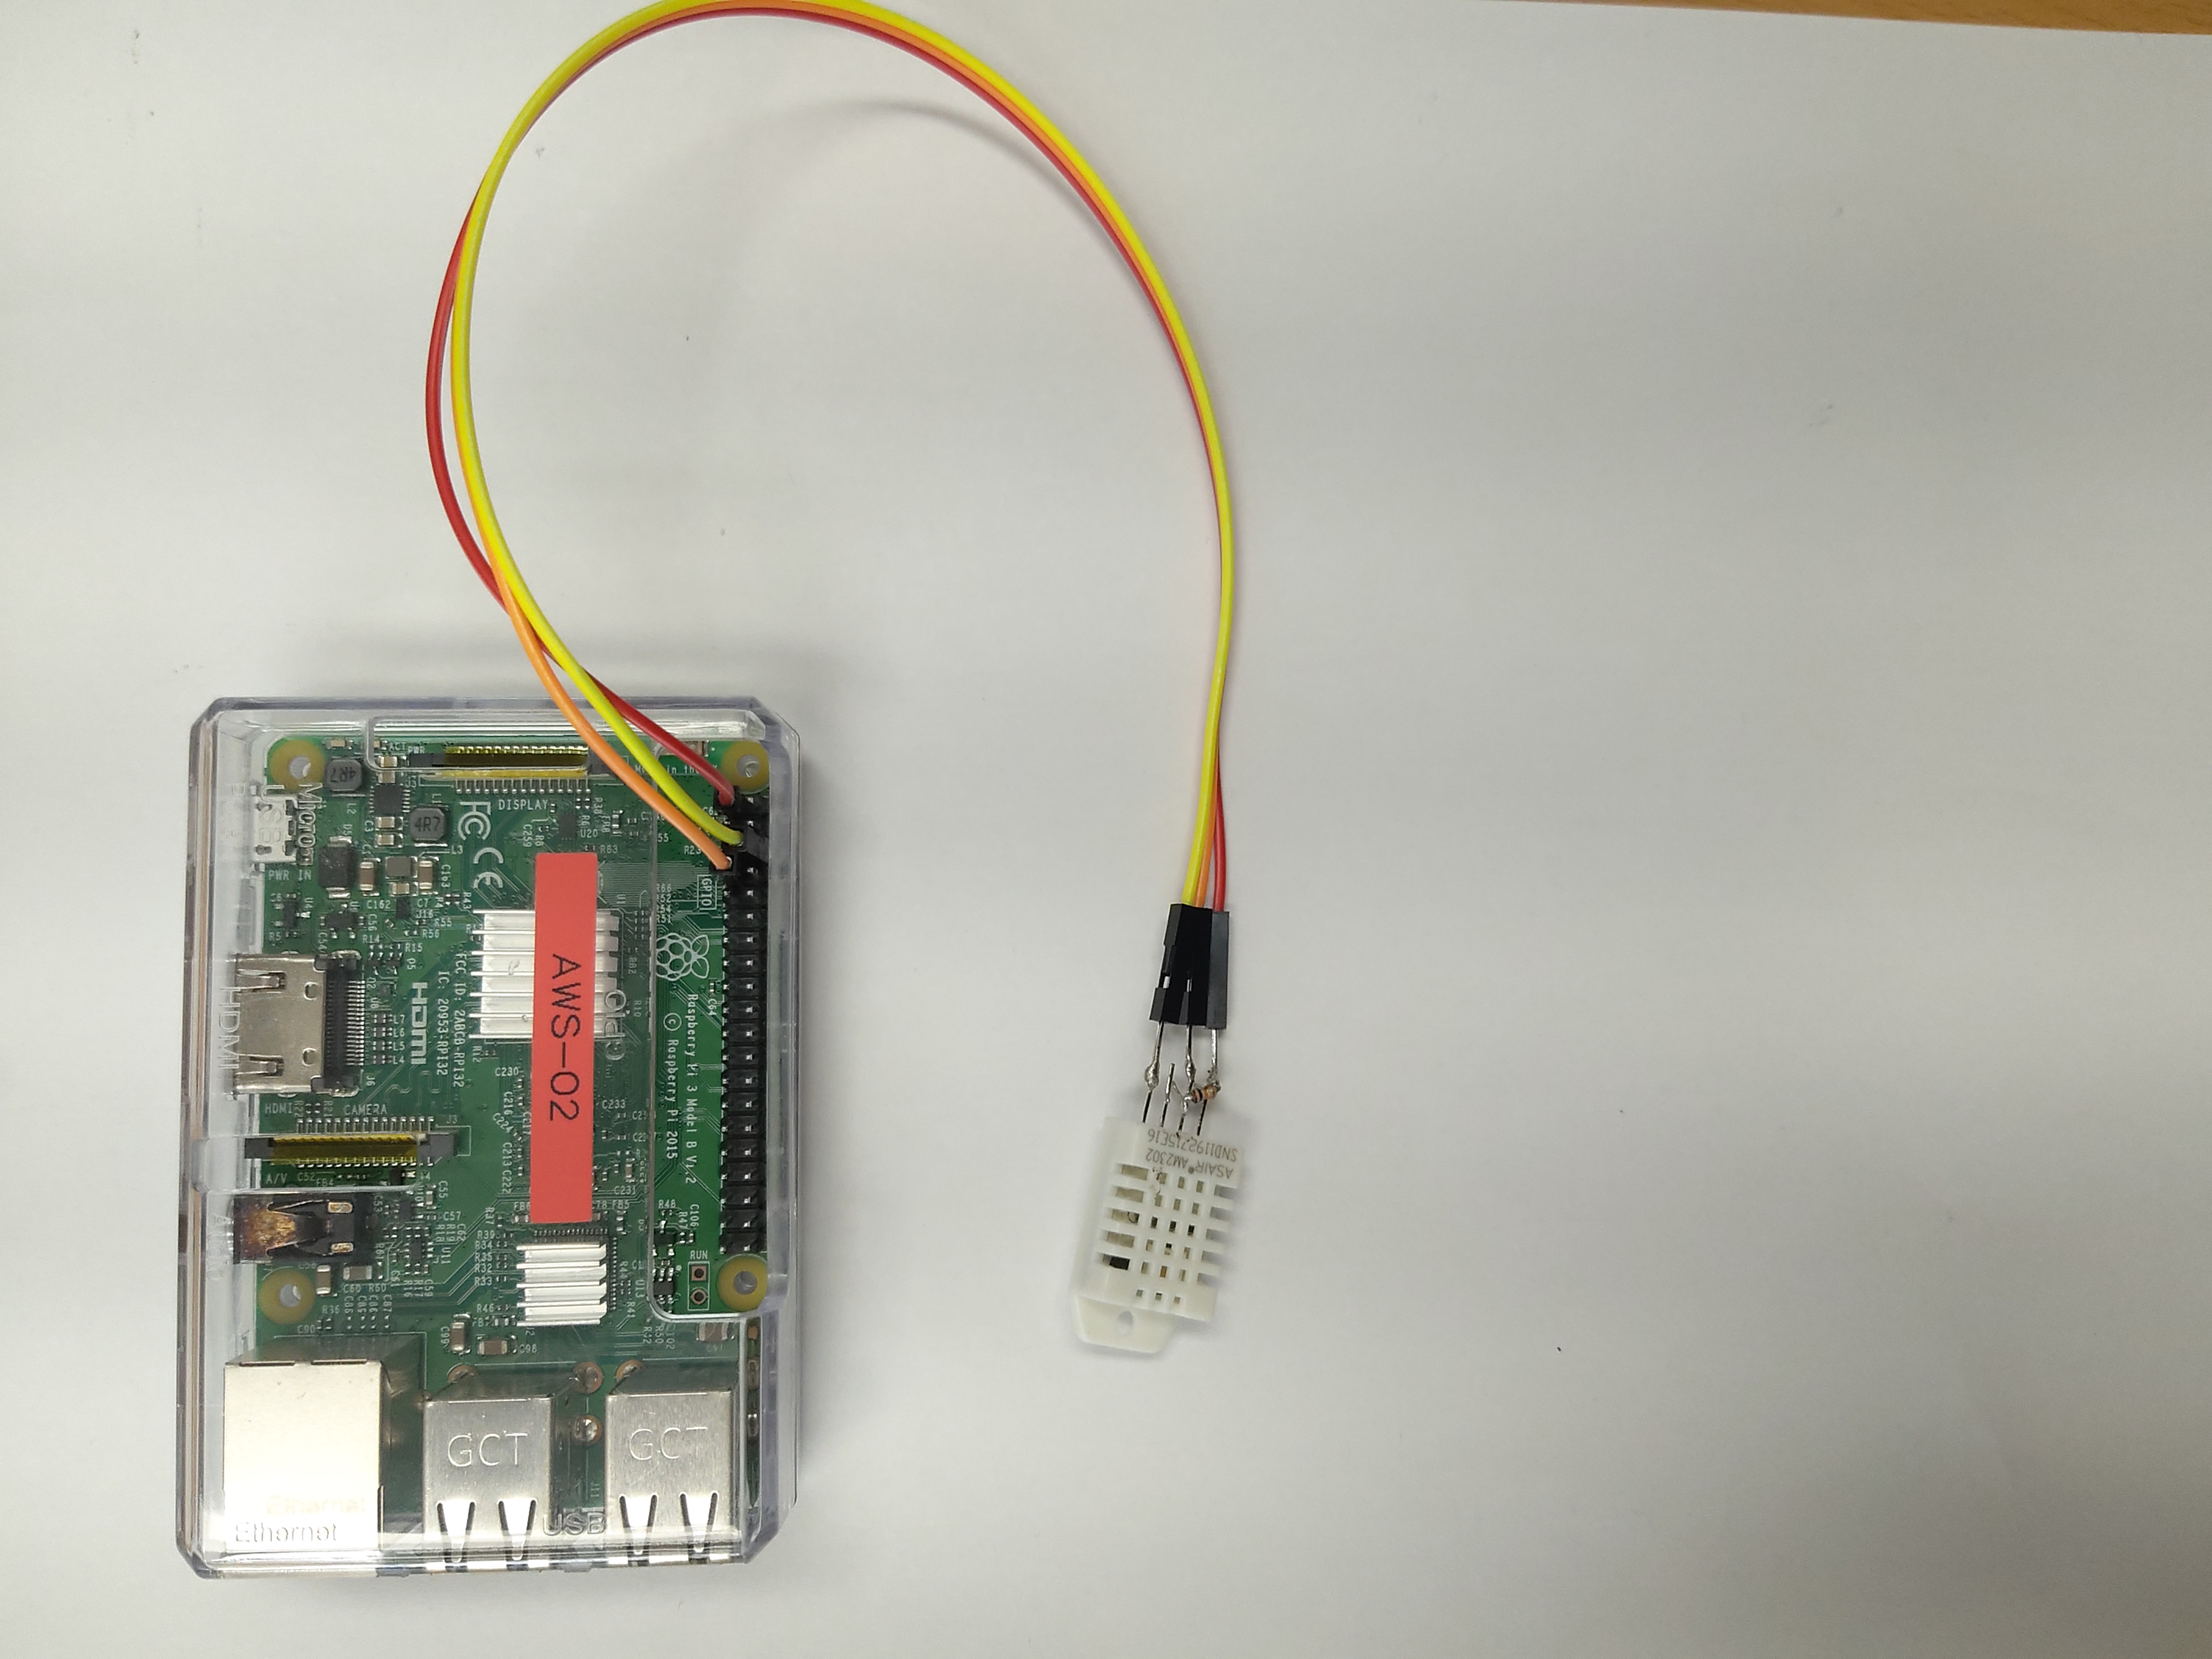
\includegraphics[width=.6\textwidth]{dht22_connect.jpg}
	\caption{DHT22 센서를 단독으로 연결한 모습}
	\label{DHT22}
\end{figure}

\subsubsection{기압 센서(BMP180)}
BMP180은 센서가 위치한 지역의 기압값을 측정하는 센서이며, 추가로 온도도 측정 가능하지만 본 연구에서는 이미 온습도 센서가 존재하기에 온도를 표출하는 기능은 사용하지 않았다. BMP180은 3.3V의 입력 전압을 요구하며 2가지 방법으로 배선이 가능하다. BMP180의 통신에는 SPI(Serial Peripheral Interface Bus) 통신을 사용하는 방법과 I2C(Inter-Integrated Circuit) 통신을 사용하는 방법이 존재하였으며 두 방법 모두를 사용하여 연결을 시도해 보았다.
\subsubsection*{SPI 통신 사용}
아래 배선도와 같이 선을 연결하여 사용한다. 3.3V 핀 1개, 디지털 출력 핀 4개, GND 핀 1개를 요구하며 Python 코드의 실행을 위해 라이브러리를 라즈베리파이에 설치하였다. 코드는 센서에서 받아들인 값을 기압(hPa 단위)와 해발고도(m 단위)로 환산하여 출력하며 온도도 섭씨온도 단위로 출력한다.

\begin{figure}[htbp]
	\centering
	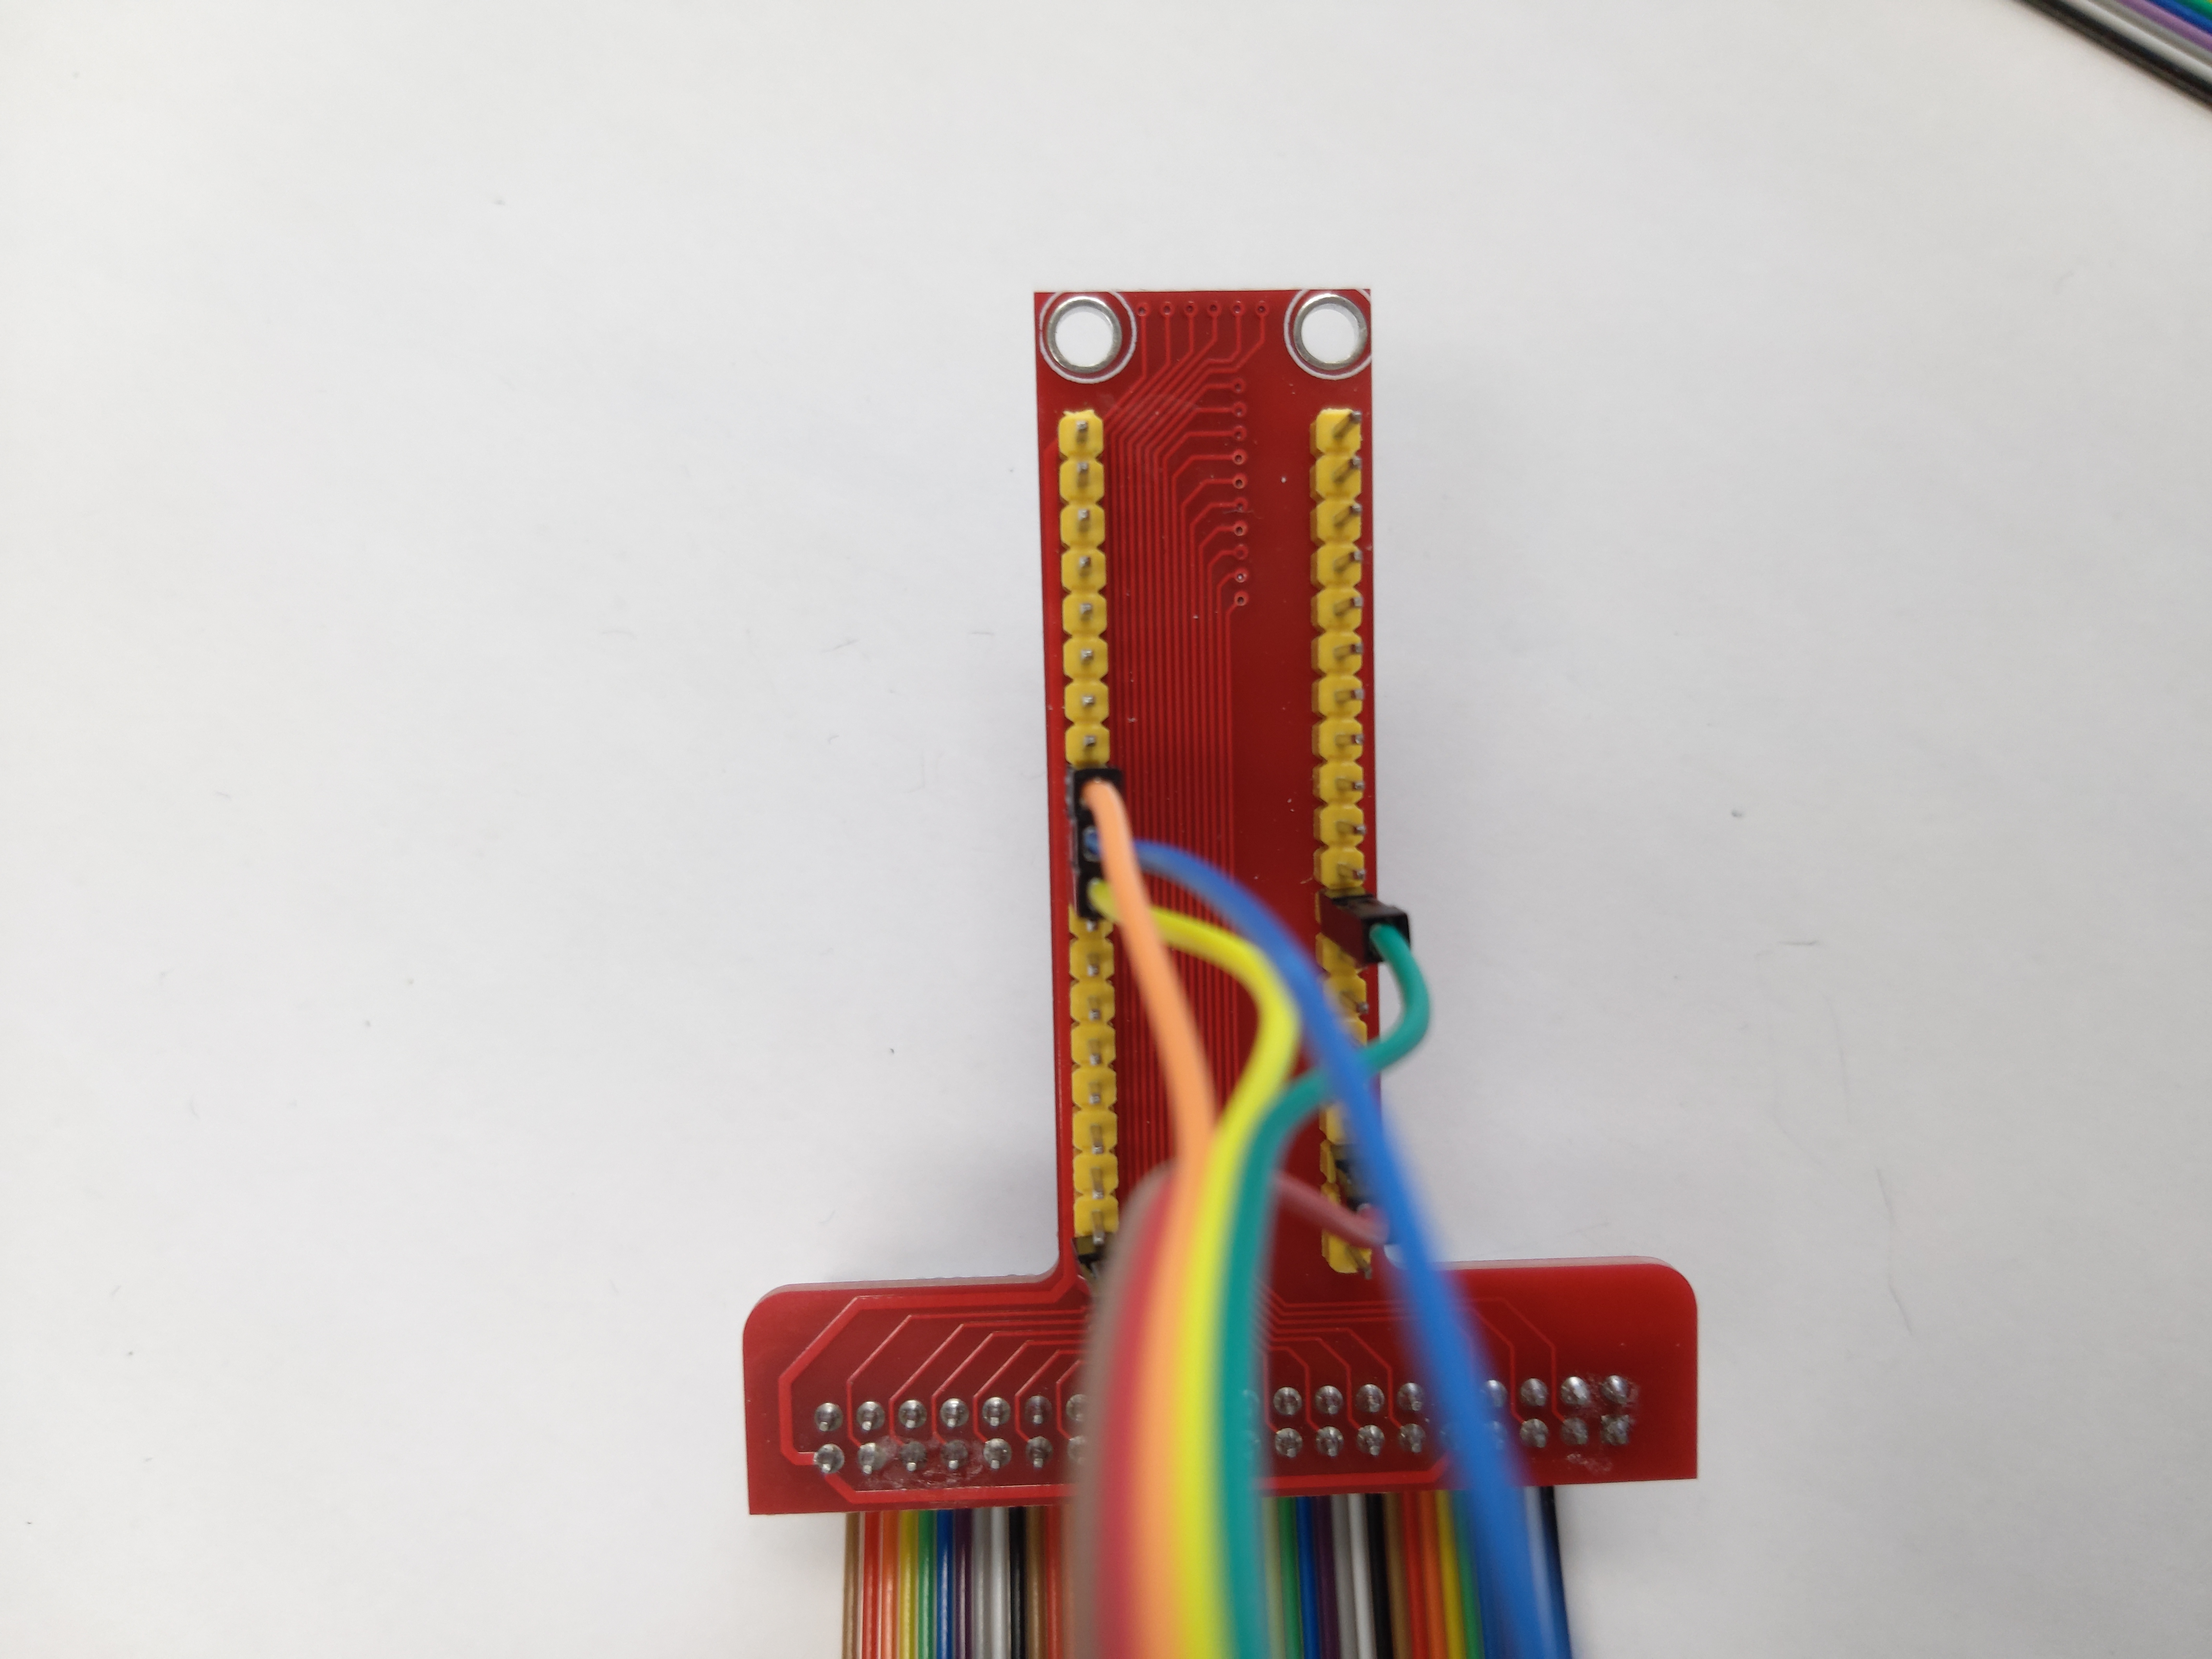
\includegraphics[width=.45\textwidth]{spitest_1}
	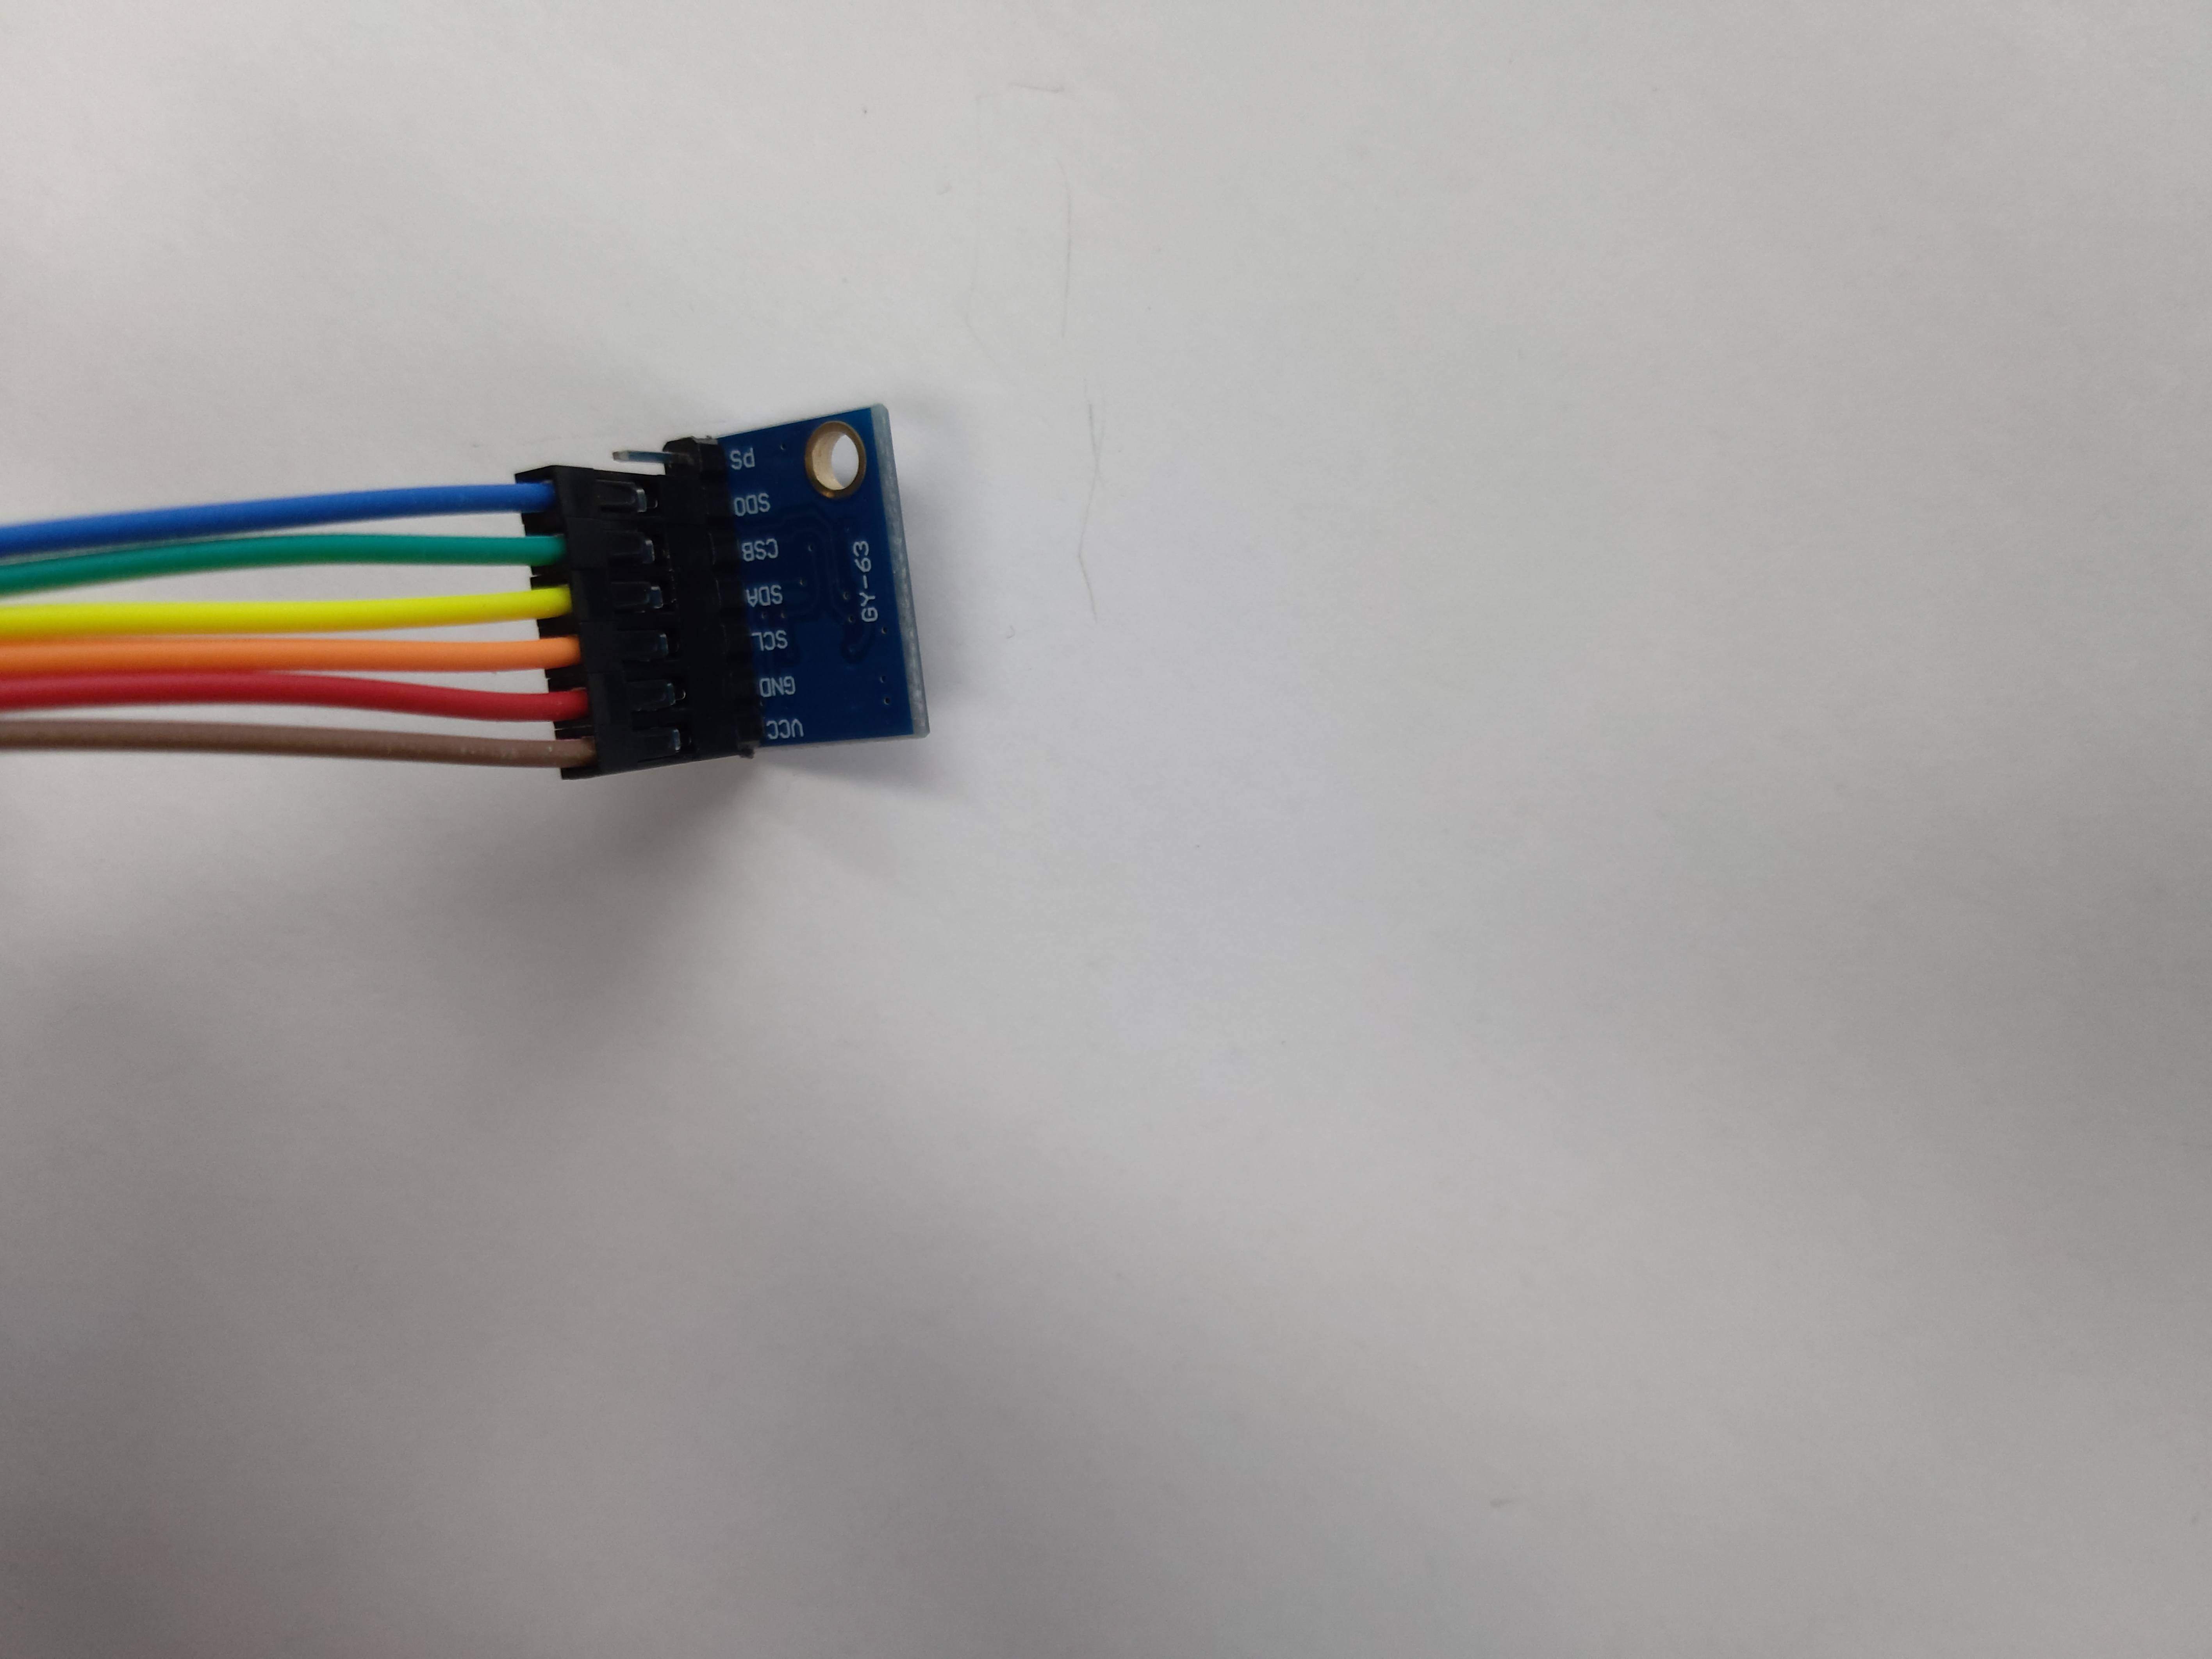
\includegraphics[width=.45\textwidth]{spitest_2}
	\caption{SPI 통신을 사용한 BMP180 센서의 연결}
	\label{SPI}
\end{figure}

\subsubsection*{I2C 통신 사용}
아래 배선도와 같이 전선을 연결한다. 3.3V 핀 1개, GND 핀 1개와 디지털 출력 핀 2개를 사용하며 나머지 핀은 연결하지 않는다. Python 라이브러리를 설치 후 코드를 구동해 센서에서 받아들인 값을 기압(mba 단위)와 온도(섭씨온도 단위)로 출력하였다.

\begin{figure}[htbp]
	\centering
	\includegraphics[width=.6\textwidth]{pressure}
	\caption{I2C 통신을 사용한 BMP180 센서의 연결}
	\label{I2C}
\end{figure}

\subsubsection{미세먼지 센서(PMS7003)}
미세먼지 센서는 공기 중의 미세먼지 농도를 측정하는 센서이다. 미세먼지는 공기 중에 떠다니는 부피 10㎛³ 이하의 작은 먼지 입자를 일컬어 부르는 말이며 크기가 작아 인체에 흡수된 후 쉽게 제거되지 않아 각종 호흡기 질환을 일으키는 원인이기도 하다. 본 미세먼지 센서는 공기 중 미세먼지에 의해 빛이 산란되는 원리를 이용해 미세먼지의 대기 중 농도를 측정하나 이는 단위 부피당 질량이 아닌 입자수로 출력되기 때문에 미세먼지의 평균 질량에 입자수를 곱해 단위부피당 미세먼지의 질량을 구한다. 미세먼지 센서는 UART 통신 방식을 사용하기 때문에 GPIO 핀을 사용하여 연결하지 않으며, USB to TTL을 사용해 센서에 전선을 연결하고 그 전선을 케이블을 통해 라즈베리파이의 USB 포트에 연결하여 값을 수신한다. 라즈베리파이 3에서 UART 통신은 기본적으로 비활성화되어 있기 때문에 이를 사용하기 위해서는 환경설정에서 활성화시켜줘야 하며, 이 과정은 라즈베리파이의 블루투스 통신을 비활성화시키는 과정을 포함한다.
미세먼지 센서에 인터페이스 보드를 결합한 후, 아래 그림과 같이 4개의 전선을 연결한다. 그리고 이 전선을 USB to TTL 케이블에 연결한 후, 케이블을 라즈베리파이에 연결한다. 그 후 미세먼지서버가 연결된 UART를 확인하고 Python 코드에서 UART명을 입력하는 부분에 현재 센서가 연결된 UART를 입력한다. 결과값 표출 명령어는 PMS7003의 데이터시트와 제공되는 예시 코드를 변형하여 사용한다.

\begin{figure}[htbp]
	\centering
	\includegraphics[width=.6\textwidth]{pms7003_connect.jpg}
	\caption{PMS7003 센서를 USB to TTL 케이블을 사용해 연결한 모습}
	\label{PMS7003}
\end{figure}

\subsubsection{ADC(Analog to Digital Converter, MCP3208)}
풍향센서와 풍속센서는 각각 바람의 세기와 방향에 따라 결과를 전압 값으로 출력하며 이 값을 읽어들이기 위해서는 아날로그 통신이 필요하다. 그러나 라즈베리파이의 GPIO 핀 중에는 아날로그 통신이 가능한 핀이 없기 때문에 아날로그 신호를 디지털로 바꿔주는 ADC, 즉 아날로그-디지털 변환기를 사용해 값을 받아들인다. 본 연구에서 사용하는 ADC인 MCP3208은 아날로그 입력값을 받아들이는 8개의 핀과 그 값을 라즈베리파이에 전송하기 위해 사용하는 8개의 핀으로 구성되어 있다. ADC를 라즈베리파이에 연결하는 방법은 그림과 같으며 명령어는 C와 Python 2개의 언어를 모두 사용해 구동시켜 보았다.

\begin{figure}[htbp]
	\centering
	\includegraphics[width=.6\textwidth]{adc_connect}
	\caption{ADC(MCP3208)을 라즈베리파이에 연결한 모습}
	\label{ADCCON}
\end{figure}

\subsubsection{풍속센서(SEN0170)}
풍속센서는 바람이 흐르는 속력을 측정하는 센서이다. 풍속센서의 풍속계는 바람이 세게 불수록 더 빨리 회전하며, 센서는 이 회전하는 정도를 연속적인 전압값으로 출력한다. SEN0170의 데이터시트에는 풍속이 0m/s일 때 출력 전압이 0.4V, 32.4m/s 풍속일 때의 출력 전압이 2.0V로 표시되어 있었다. 32.4m/s는 본 센서가 측정할 수 있는 최대 풍속이며 그러므로 출력되는 최대 전압은 2.0V를 넘지 않는다. 본 연구에서는 전압과 풍속의 상관관계가 선형적이라고 가정한 뒤 전압에 따른 풍속을 구하는 공식을 도출하였다. 전압을 $V$[V], 풍속을 $v$[m/s]라 할 때 둘 사이에는
\[ v=0.25V-8.1\quad (V\geq 0.4)\]
의 관계가 성립함을 알 수 있었다. 이때 전압이 0.4V 미만이라면 풍속은 0m/s로 표시하도록 하였다.
풍속센서에는 4개의 전선이 존재한다. 2개는 각각 (+)와 GND를 연결하는 전선이며, 1개는 전압을 출력하는 전선이고, 나머지 1개의 전선은 사용하지 않는다. 데이터시트에 의하면 풍속센서는 7~24V의 직류 전압 사이에서 동작하므로 12V 배터리에 센서를 연결하여 사용하기로 하였다. (+)극 선과 GND 선을 12V 배터리에 연결할 수 있도록 케이블과 납땜하였으며, 풍속센서의 출력 전선을 ADC의 CH0(아날로그 전압값을 읽어들이는 핀)에 연결한 후 명령어를 작성하고 실행해 풍속이 올바르게 표출되는지 확인하였다. 명령어는 ADC에서 사용한 코드에서 읽어들인 전압값을 이용해 풍속을 계산하여 출력하도록 하였다.

\subsubsection{풍향센서(DM2014)}
풍향센서는 바람이 부는 방향을 출력하는 센서이다. 데이터시트에 의거하면 풍향센서는 바람이 부는 방향에 따라 16방위로 나누어 각 방위에 따라 전압값을 다르게 표현하며, 이를 이용해 바람이 불어오는 방향을 알 수 있다. 풍향센서에는 4개의 핀이 존재하며 2개는 각각 (+)극과 GND를 연결하는 선이고 1개는 전압을 출력하는 전선, 나머지 1개는 사용하지 않는 전선이다. 풍향센서의 동작전압은 12~24V 사이의 직류 전압이므로 (+)극 선과 GND 선이 배터리에 연결될 수 있도록 전선을 케이블에 납땜한 뒤 12V의 배터리에 풍향센서를 연결한다. 명령어를 작성하고 구동하기 전에 멀티미터를 사용하여 바람의 방향이 변함에 따라 전압값이 제대로 출력하는지 확인하였다. 멀티미터를 사용하여 GND 핀과 출력 전압 핀 사이의 전압을 측정하였다.

\begin{figure}[htbp]
	\centering
	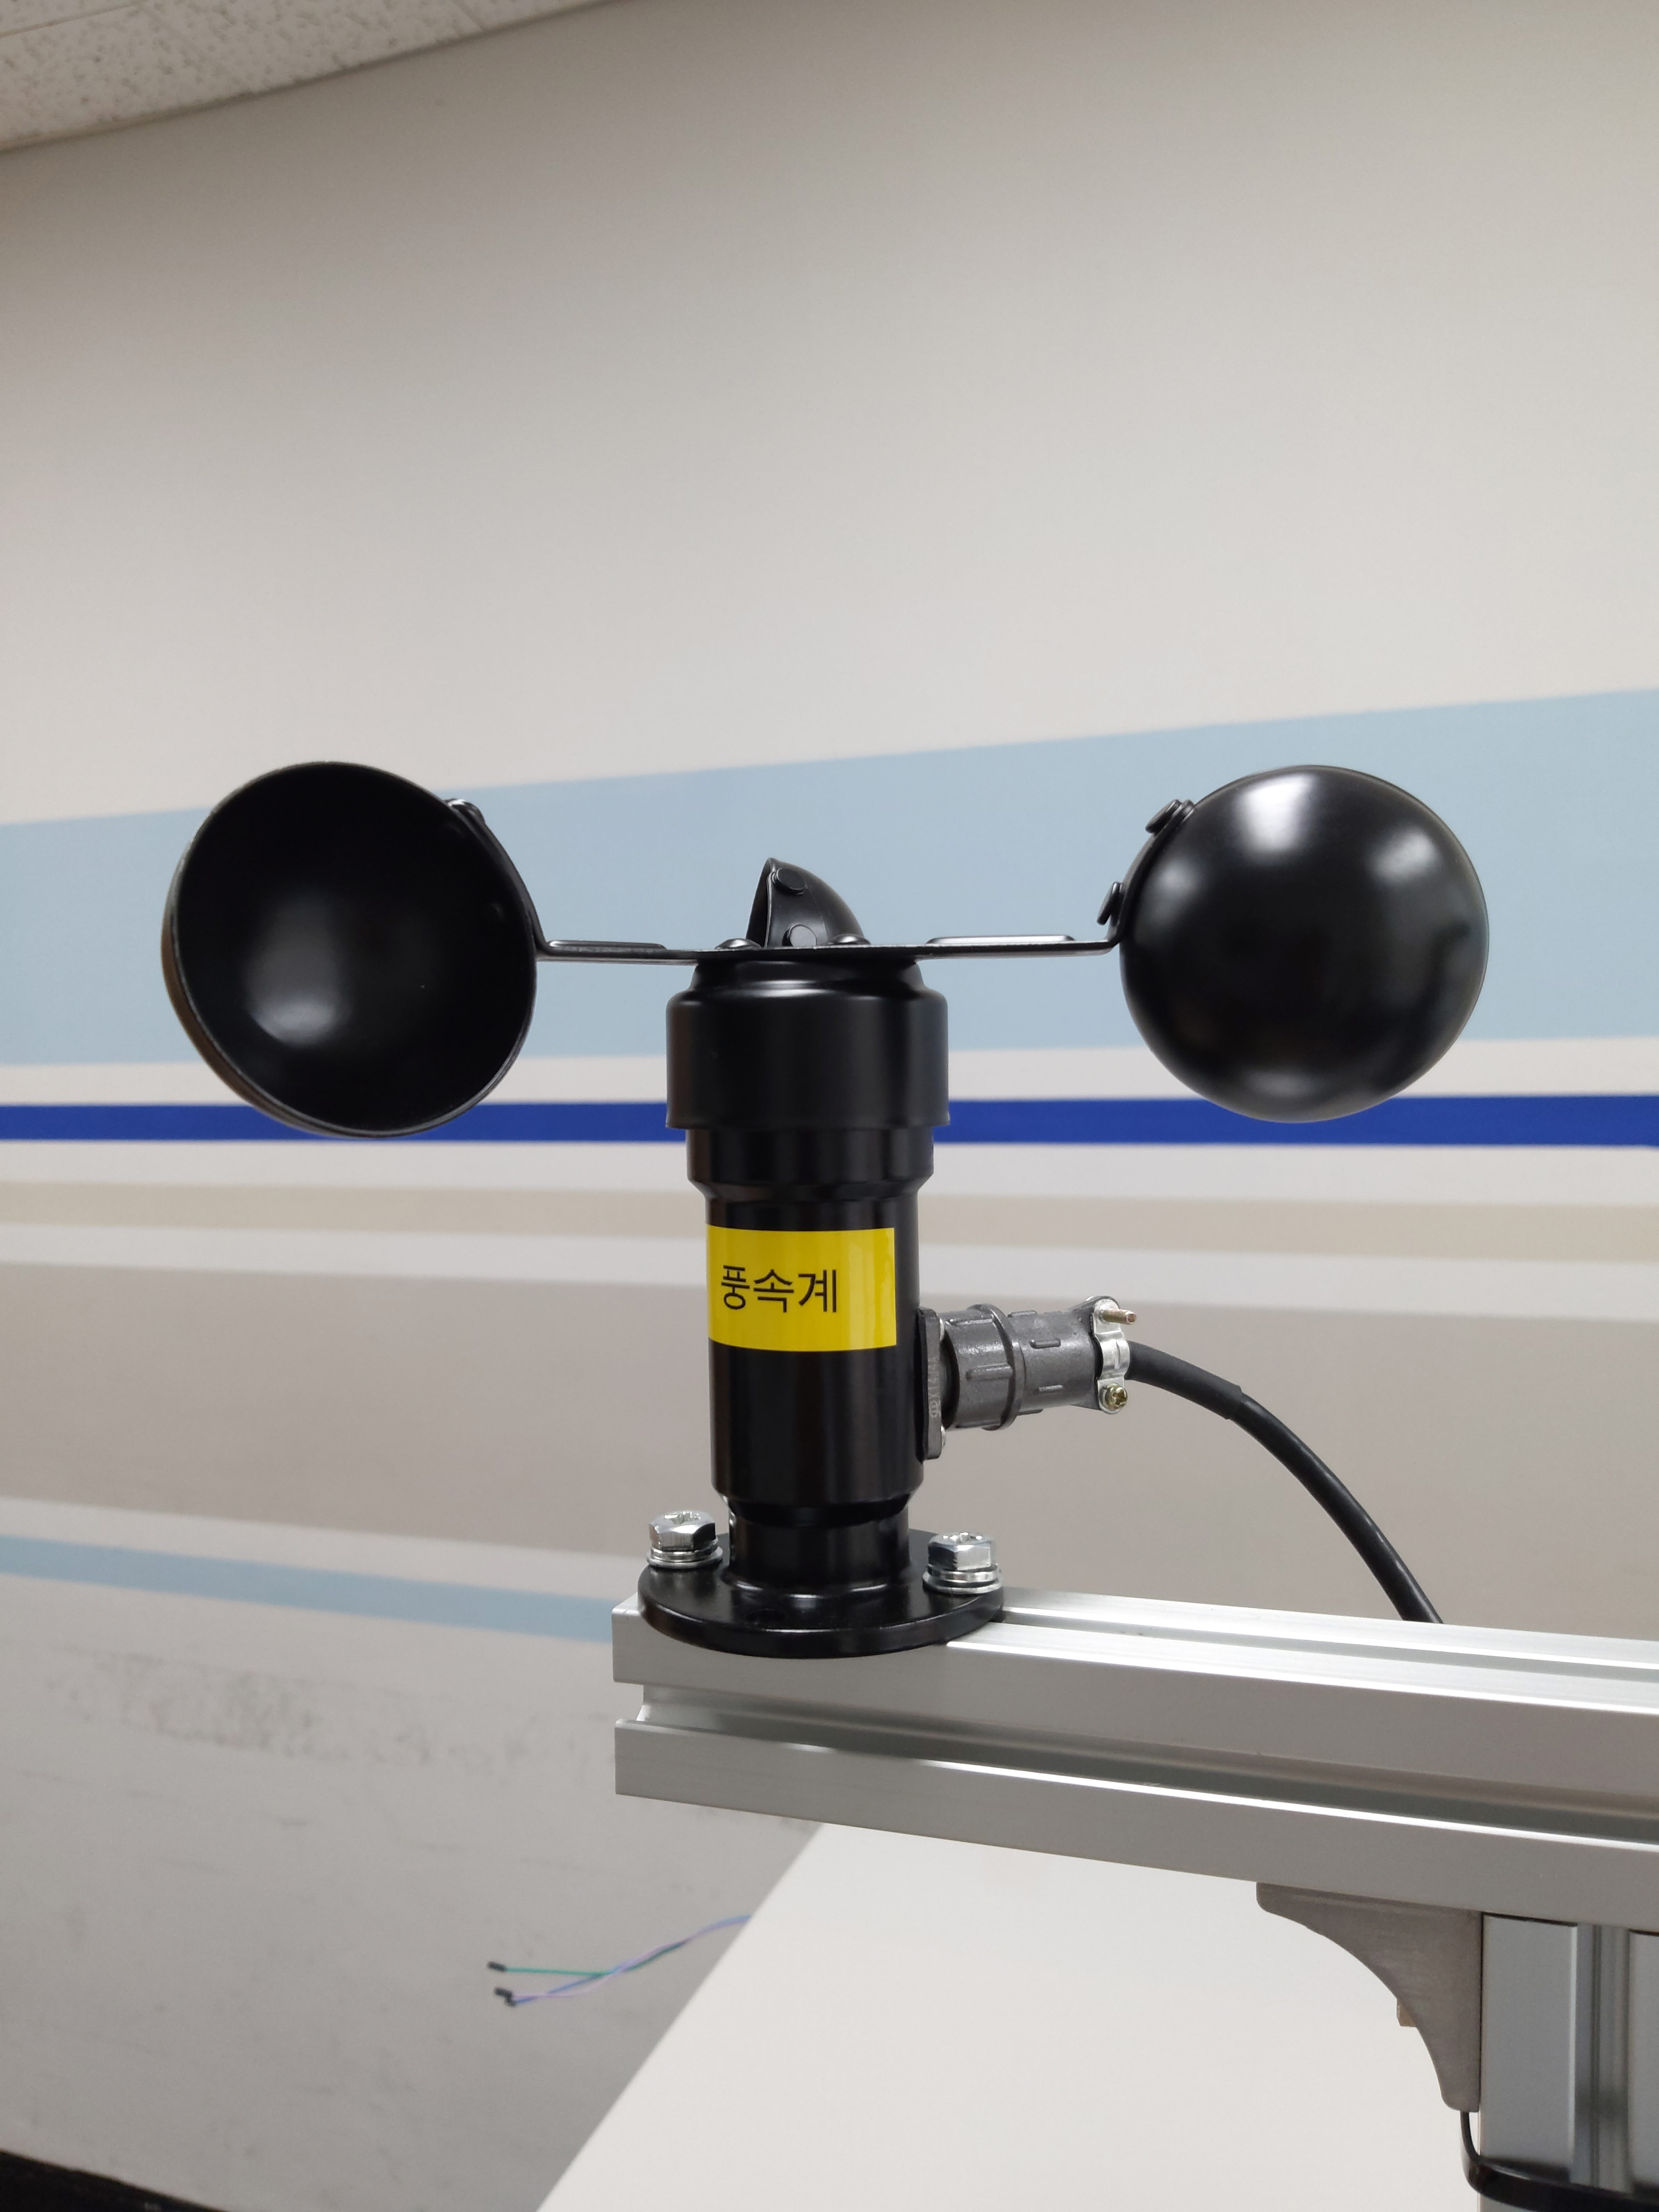
\includegraphics[width=.45\textwidth]{windspeed}
	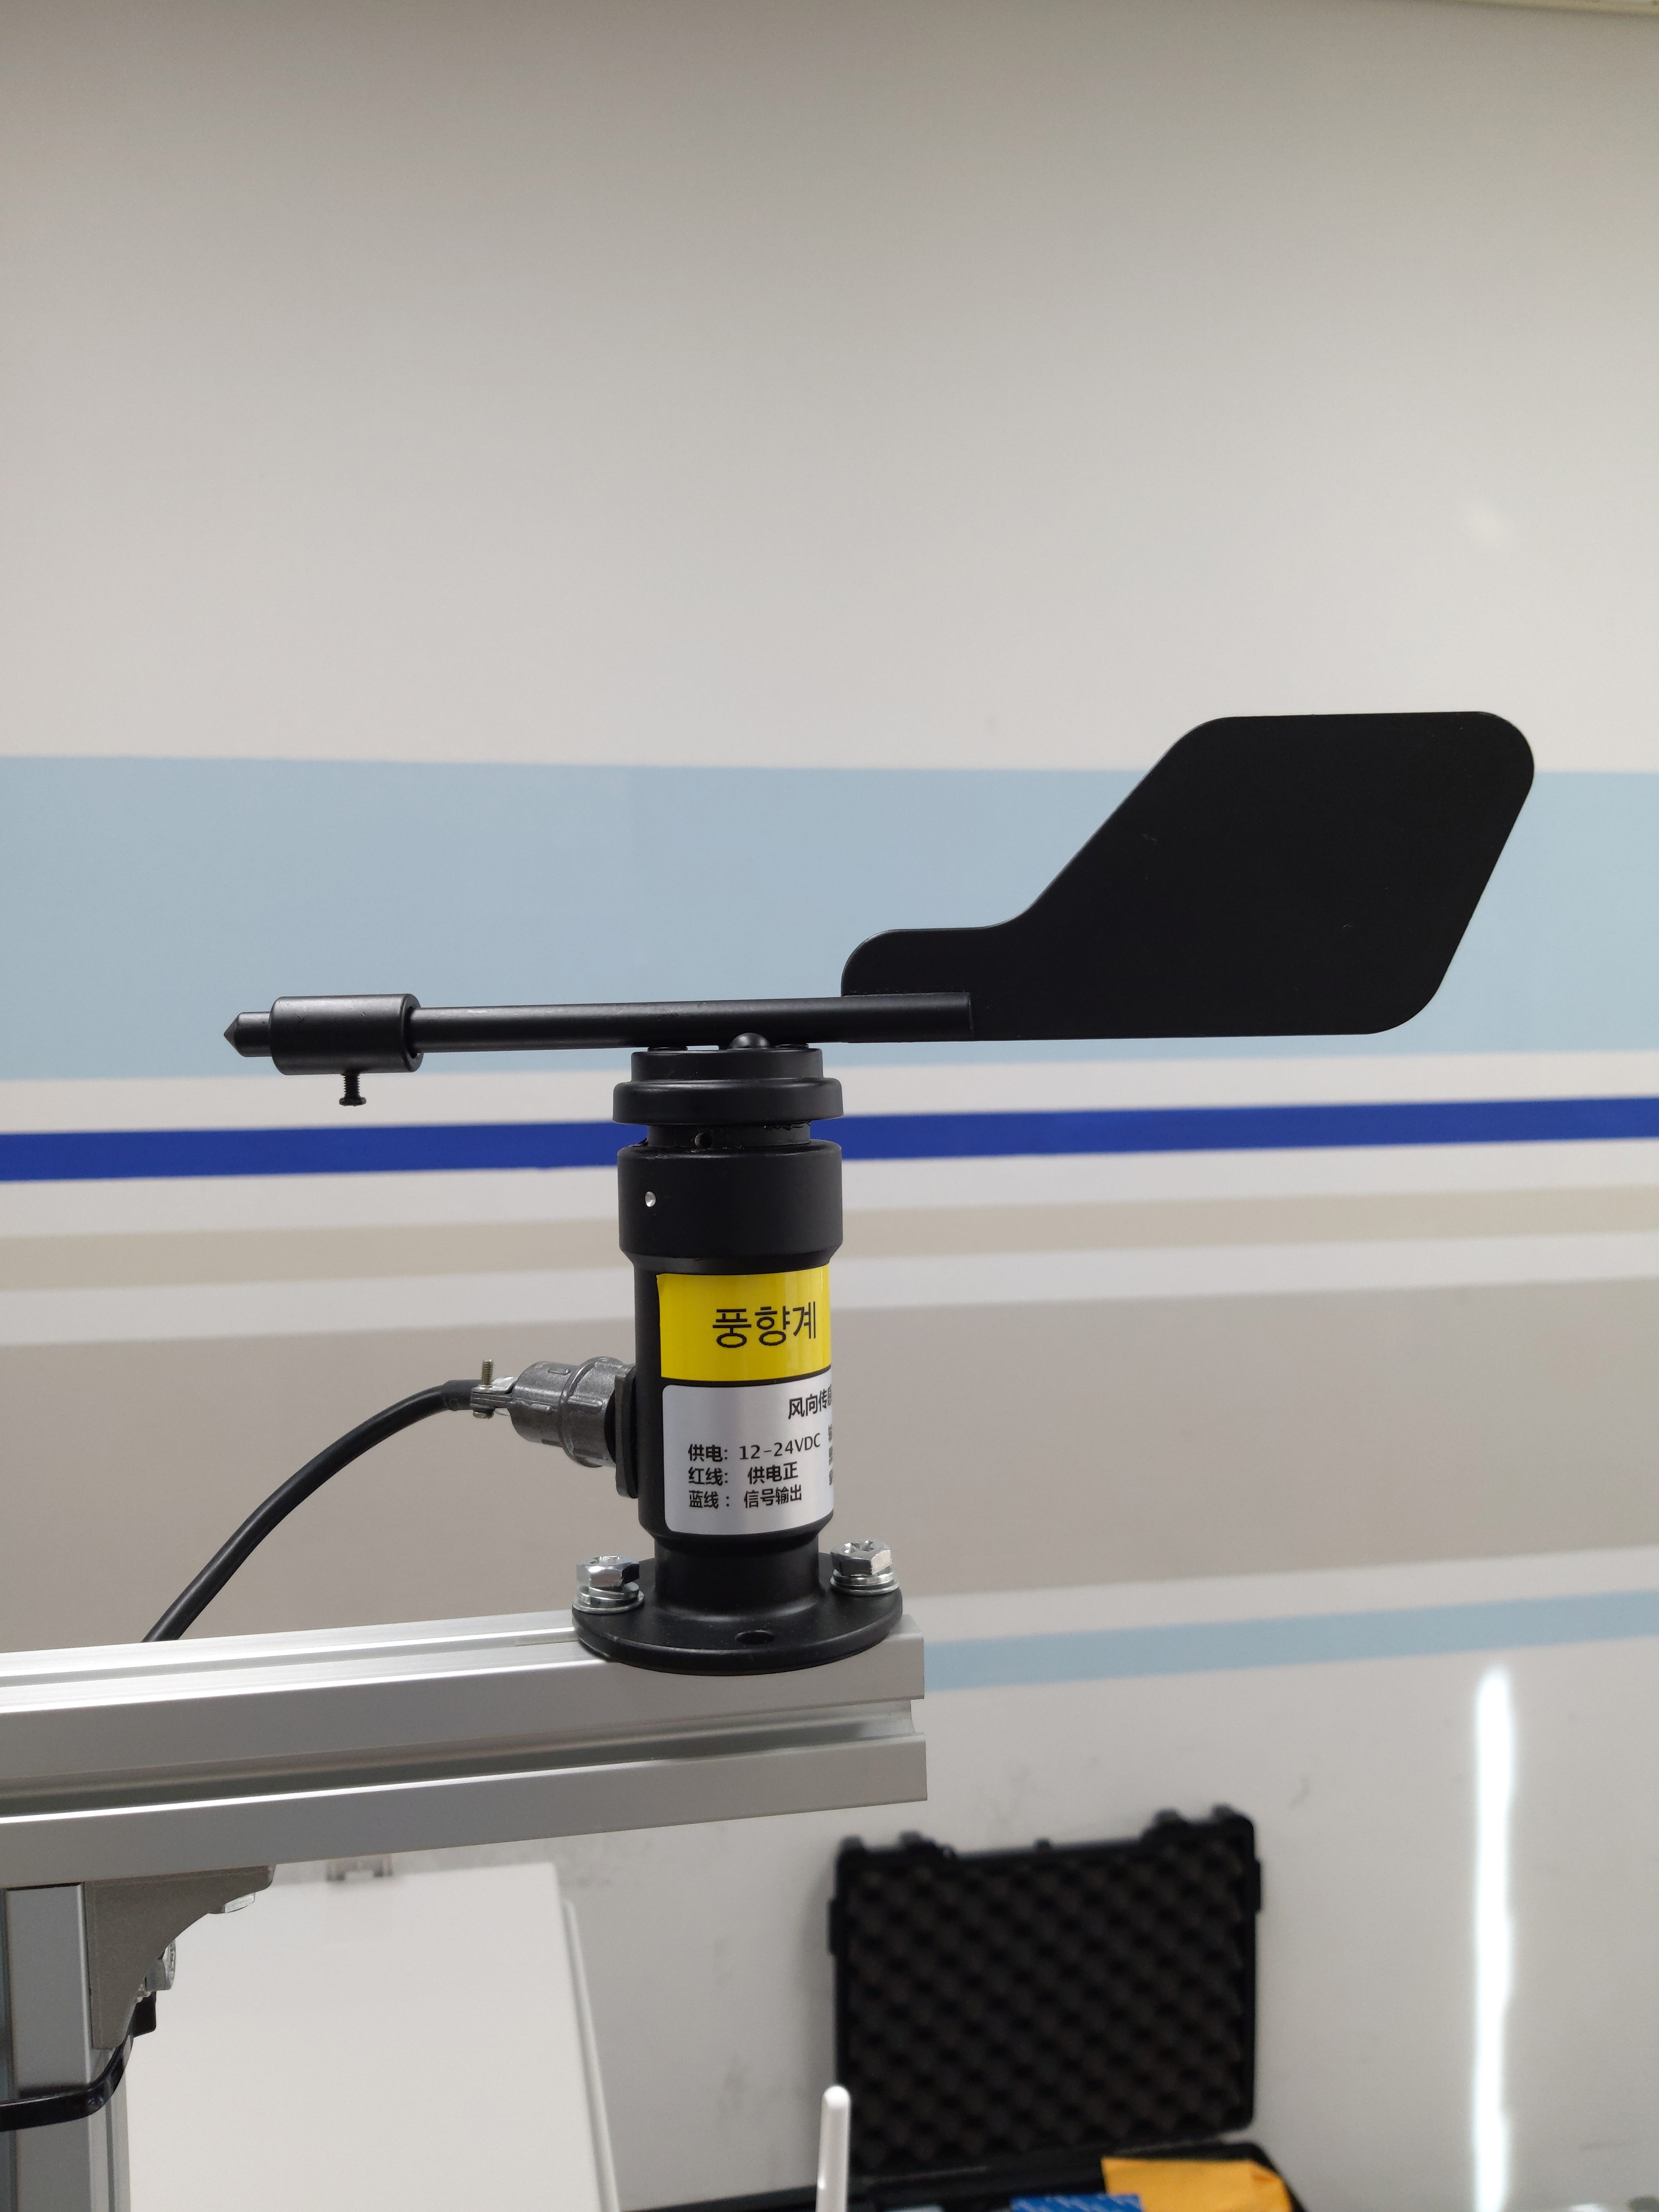
\includegraphics[width=.45\textwidth]{winddir}
	\caption{풍속센서와 풍향센서의 모습}
	\label{WIND}
\end{figure}

\subsubsection{강우량센서(p/n 80422)}
강우량센서는 빗방울이 떨어질 때만 신호가 전달되는 방식으로 강우량을 측정한다. 강우량센서에 빗방울이 떨어지면 강우량센서의 하부에 위치한 시소 모양의 건축물이 기울어지게 된다. 이에 따라 버튼이 눌려지고 버튼이 한 번 눌려질 때마다 신호가 전달되는 방식이다. 센서는 강우량을 비 한 방울의 부피와 버튼이 눌러진 횟수를 곱해 구한다. 강우량 센서의 전선을 다음과 같이 연결한 후 명령어를 작성해 실행 여부를 확인한다. 강우량 센서에 빗방울이 떨어진 경우에만 프로그램이 값을 출력하게 되어 있다.

\begin{figure}[htbp]
	\centering
	\includegraphics[width=.6\textwidth]{rainfall}
	\caption{강우량센서를 라즈베리파이에 연결한 모습}
	\label{RAINFALL}
\end{figure}

\subsection{AWS 구조물의 보수와 센서의 기판 연결}
본교의 SRC(Science Research Center) 7층 야외에 위치해 있으나 현재 사용하지 않는 AWS 구조물을 보수하고 센서와 전선을 연결했다. AWS 구조물은 알루미늄 프로파일을 이용해 제작하였으며 양쪽 벽면에 와이어를 이용해 고정하였으나 과거 붕괴되어 추가적인 보수가 필요한 상황이었다. 본 연구에서는 알루미늄 프로파일의 접합부에 볼트와 너트를 2중으로 설치하였으며, 구조물의 양쪽을 와이어를 사용해 벽에 단단하게 고정하였다. 또한 구조물의 상단부에 풍속 센서와 풍향 센서를 설치하고 전선을 케이블 타이로 알루미늄 프로파일에 고정하였다. 구조물의 중간 부분에는 라즈베리 파이와 배터리, 풍향, 풍속, 강수량을 제외한 각종 센서가 위치할 공간이 위치해 있다. 상자에 라즈베리 파이와 온습도, ADC, 기압 센서를 연결한 기판을 놓은 후 상자에 펀치를 이용해 전선이 들어갈 구멍을 뚫는다. 배터리와 상자를 구조물 위에 놓은 후 풍속, 풍향, 강우량 센서의 전선과 배터리의 전선을 상자 안에 넣어 라즈베리파이와 연결한다.
풍향과 미세먼지 센서를 제외한 모든 센서의 전선과 ADC, 라즈베리파이 확장 보드를 만능기판에서 서로 납땜하여 연결한다. 라즈베리파이 확장 보드는 라즈베리파이에 연결하였을 경우 라즈베리파이에 기본적으로 내장되어 있는 핀과 동일한 용도로 사용할 수 있으며 전선의 연결과 납땜, 이후 유지 보수를 쉽게 해주는 역할을 한다.

\subsection{서버 데이터베이스로 수집한 정보 전송}
MariaDB를 통해 수집한 기상 정보를 체계적으로 정리할 데이터베이스를 구축한 후 이를 웹상에서 관리하기 위해 경기과학고 지구과학 홈페이지(ess.gs.hs.kr)에 설치된 phpMyAdmin을 이용하였다. 서버에 기상 정보를 저장하는 DB인 AWS\_GSHS를 만든 후 아래와 같이 테이블을 제작하였다. 테이블의 이름은 1min\_data로 하였으며 내용은 기상청 날씨누리에서 제공하는 AWS 관측자료의 형식을 따랐으며 본 연구에서 제작한 AWS 장비에서 현재 측정할 수 없는 자료는 NULL값을 기본으로 저장하기로 설정하였다.
라즈베리파이에서 수집한 값을 서버에 전송하기 위해 Python에서 pymysql 모듈을 불러온 후 SQL문을 사용한다. C언어와 Python 명령어에서 반복문을 실행하는 시간 간격이 같도록 프로그램의 시간 딜레이를 설정하였다. 또한 수집한 정보는 라즈베리파이 내부에도 csv 파일의 형태로 저장하도록 설정하였다.

% Please add the following required packages to your document preamble:
% \usepackage{graphicx}
\begin{table}[]
	\caption{AWS\_GSHS DB의 1min\_data 테이블 구조}
	\label{DBTable}
	\resizebox{\textwidth}{!}{%
		\begin{tabular}{|c|c|c|c|c|}
			\hline
			이름            & 설명            & 데이터형    & 기본값  & 비고            \\ \hline
			id            & 데이터 일련번호      & int     &      & 자동으로 부여       \\ \hline
			OBS\_code     & AWS 지역코드      & int     &      & 임의로 111111 부여 \\ \hline
			OBS\_datetime & 측정시각          & varchar &      & 연월일-시분초로 표시   \\ \hline
			preci\_now    & 현재 강수여부       & varchar &      & O, X로 표시      \\ \hline
			preci\_15     & 15분 누적강우량     & float   &      &               \\ \hline
			preci\_60     & 60분 누적강우량     & float   &      &               \\ \hline
			preci\_3H     & 3시간 누적강우량     & float   &      &               \\ \hline
			preci\_6H     & 6시간 누적강우량     & float   &      &               \\ \hline
			preci\_12H    & 12시간 누적강우량    & float   &      &               \\ \hline
			preci\_1day   & 1일 누적강우량      & float   &      &               \\ \hline
			temperature   & 기온            & float   &      &               \\ \hline
			wind\_dir011  & 1시간 풍향(360도)  & float   & NULL &               \\ \hline
			wind\_dir012  & 1시간 풍향(16방위)  & float   & NULL &               \\ \hline
			wind\_spd01   & 1시간 풍속        & float   &      &               \\ \hline
			wind\_dir101  & 10시간 풍향(360도) & float   & NULL &               \\ \hline
			wind\_dir102  & 10시간 풍향(16방위) & float   & NULL &               \\ \hline
			wind\_spd10   & 10시간 풍속       & float   & NULL &               \\ \hline
			RH            & 상대습도          & float   &      &               \\ \hline
			Air\_P        & 대기압           & float   &      &               \\ \hline
			REMARK        & 비고            & varchar &      & ‘RnE’로 표시     \\ \hline
		\end{tabular}%
	}
\end{table} % 원래 있던 문
	\section{결과 및 토의}

우선 온습도센서는 프로그램을 실행하였을 때 정상적으로 온도와 습도가 표현됨을 알 수 있었으나 기압센서는 SPI 통신을 사용하였을 때 기압이 약 390hPa 정도로 실제와 전혀 맞지 않는 값이 출력되었다. 센서를 교체하여도 같은 현상이 일어났고 센서에서 값을 받아오는 것 자체에는 문제가 없는 것으로 판단되었으므로 센서에서 받아온 값을 기압으로 출력하는 명령어에 문제가 있던 것으로 추정된다. 그러나 SPI 통신은 ADC가 사용하여야 하고 라즈베리파이 하나에는 기본적으로 한 세트의 SPI 통신 판만이 존재하기에 대신 I2C 통신을 사용하여 기압센서를 연결하였으며, 그 결과 기압이 1000mba 내외로 정상적으로 표출되어서 기압 값을 수집할 때 I2C 통신을 사용하기로 하였다. 

미세먼지 센서의 경우 프로그램이 실행된 이후 몇 초 동안은 값이 정상적으로 표출되었으나 그 후 원인불명의 오류와 함께 프로그램이 정지하였다. UART 통신에서 값을 받아오는 부분에 문제가 있던 곳으로 추정되며 일반적인 자동기상관측장비에서는 미세먼지 농도를 측정하지 않기에 AWS에 미세먼지 센서는 일단 설치하지 않는 것으로 결정하였다. 

ADC의 경우 C언어와 Python으로 컴파일된 프로그램 두 개를 각각 실행한 결과 Python 코드의 경우 오류는 발생하지 않으나 센서의 연결 여부와 무관하게 전압이 계속 0으로 측정되는 문제가 있었다. 반면 C언어 코드의 경우 전압이 정상적으로 출력되었다. AWS를 구동하는 전체 명령어는 Python으로 작성하였으므로 C언어에서 파일 입출력을 통해 텍스트 파일에 수집한 전압 값을 Python에서 다시 한 줄씩 읽어들이는 방법을 선택하였다. 풍속 센서의 경우 라즈베리파이에 (+)극과 GND를 연결하지 않으며 오로지 출력 전압을 연결하는 핀 하나만 ADC에 연결한다. 

그렇기 때문에 라즈베리파이에 전원을 공급하는 배터리와 풍속 센서에 전원을 공급하는 배터리가 같아야 두 장치에 연결된 GND의 전위가 같아 값이 정상적으로 표현된다. 1.5V 건전지의 (-)극은 라즈베리파이의 GND에, (+)극은 ADC에 연결하였을 때 약 1350mV 정도의 값이 출력되었으며 건전지의 내부 저항을 고려하면 타당한 값으로 생각된다. 

풍속 센서의 출력 전압이 0.4V일 때의 풍속이 0m/s임이 데이터시트에 명시되어 있었으므로 0.4V 전압 이하에서의 풍속을 0으로 가정하였다. 풍향 센서의 경우 12V 전원을 공급한 후 풍향계가 향하는 방향을 달리한 뒤 멀티미터를 사용하여 배터리의 GND와 출력 핀 사이의 전압을 측정한 결과 방향과 무관하게 10V 가량이 나왔다. 데이터시트에 의하면 풍향에 따라 최대 5V의 전압이 출력되어야 하므로 잘못된 값임을 알 수 있다. 

강우량 센서의 경우 물방울이 한 번 떨어질 때마다 프로그램을 실행한 이후의 누적 강우량이 정상적으로 출력되었다. 최종 프로그램을 실행하였을 때 온습도와 기압, 단위 시간당 강우량, 풍속이 MariaDB 서버 데이터베이스에 정상적으로 전송됨을 확인하였다.

\begin{figure}[htbp]
	\centering
	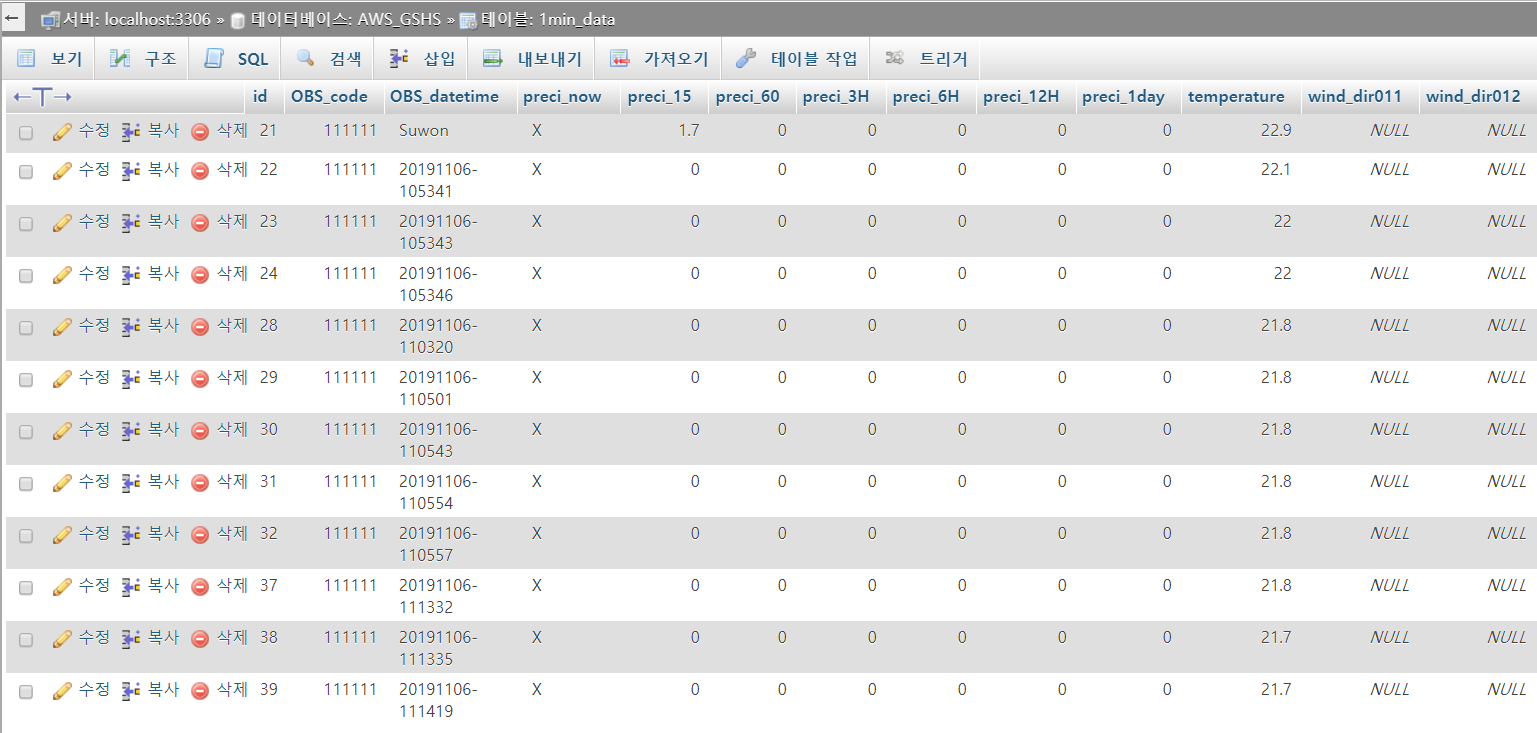
\includegraphics[width=.9\textwidth]{dbsuccess.png}
	\caption{측정한 기상 정보를 DB에 전송한 모습}
	\label{DBSENT}
\end{figure}

\begin{figure}[htbp]
	\centering
	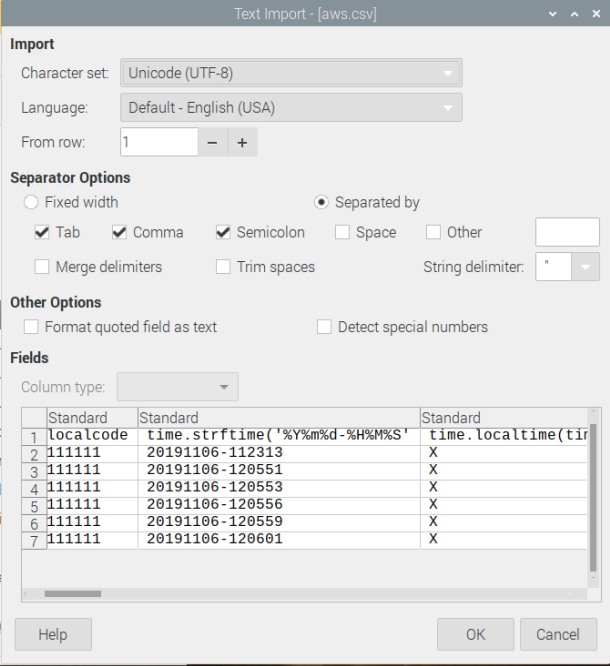
\includegraphics[width=.7\textwidth]{awscsv}
	\caption{라즈베리파이 내부 저장소에 저장된 데이터}
	\label{AWSCSV}
\end{figure}
	\section{결론}

본 연구에는 라즈베리파이와 각종 센서들을 활용하여 자동기상관측장비를 제작하고 그 자료를 서버 데이터베이스에 전송하였다. 연구 결과 대부분의 센서가 기상 정보를 정상적으로 수집하였으나 그렇지 않은 센서도 존재하였다. 기압 센서는 통신 방법에 따라 비정상적인 값이 표시되기도 하였으며, 미세먼지 센서의 경우 원인 불명의 이유로 인해 프로그램에 오류가 생겨 자료 수집이 계속 중단되었다. 풍향 센서 역시 풍향계의 방향과 무관하게 전압이 일정하게 표현되어 정보를 수집할 수 없었다. 그렇기에 추후 센서를 라즈베리파이에 연결하는 방법이나 프로그램을 변경해야 할 것으로 보이며 필요시 센서의 종류를 바꾸는 일도 필요해 보인다. 또한 센서에서 표출한 값과 실제 값이 실제로 일치하는지에 대한 확인이 필요하며 만약 차이가 보인다면 보정식을 도출하여 센서에서 수집한 값을 보정해 주어야 할 것이다. 박종서, 오완탁 (1997)의 연구에서는 자동기상관측장비와 백엽상에서 수집한 기온 값의 차이가 0.1\~{}0.4$\degree$C 정도로 측정되었으며, 하지훈, 김용혁, 임효혁, 최덕환, 이용희 (2016)는 회귀분석을 사용해 자동기상관측장비의 기압자료를 보정하는 기법을 제시하였다.\cite{Ref3}\cite{Ref4} 수집한 자료는 데이터베이스에 정상적으로 표출되었으며 이를 통해 장시간 관측으로 인해 생긴 많은 데이터를 체계적으로 관리할 수 있었으며 데이터 유실이나 훼손 등의 문제도 일어나지 않을 것으로 생각된다. 다만 기상청 날씨누리에서 제공하는 AWS 관측 자료와 비교하였을 때 본 장비에서는 수집되지 않는 기상 정보가 더 많았기 때문에 전문적인 기상 관측 자료로는 사용할 수 없으나, 온습도나 해면기압, 현재 강수 여부 등의 간단한 기상 정보는 비교적 쉽게 확인할 수 있다는 점에서 실용성이 있다고 생각된다. 또한 오류가 발생하거나 센서가 문제가 발생하였을 경우 비교적 쉽게 문제를 해결할 수 있고 센서의 가격 역시 비교적 저렴하기 때문에 AWS 장치 제작 이후의 관리 및 유지보수도 통상적인 자동기상관측장비보다 쉬울 것으로 판단된다. 또한 데이터베이스의 정보를 송죽학사 등의 교내 사이트에 정기적으로 전송해 교내 학생들이 언제나 기상 정보를 쉽고 편리하게 확인할 수 있게 하는 작업이 가능할 것으로 보인다.
	% \section{추후 연구}

\subsection{제목}

내용
	\section{부록}

\subsection{AWS Python 코드}

\lstset{basicstyle=\scriptsize, tabsize=4, numbers=left, keywordstyle=\color{blue}, commentstyle=\color{magenta}}

\begin{lstlisting}[language=python]
# Raspberry Pi ADC Python Code

# 0. Modules to import
import time
import Adafruit_DHT
import smbus
import pymysql
from gpiozero import Button

rain_sensor = Button(6)
BUCKET_SIZE = 0.2794
count = 0
count15 = 0
count60 = 0
count3h = 0
count6h = 0
count12h = 0
count1d = 0
i = 0
now15 = time.time()
now60 = time.time()
now3h = time.time()
now6h = time.time()
now12h = time.time()
now1d = time.time()
rain15 = 0
rain60 = 0
rain3h = 0
rain6h = 0
rain12h = 0
rain1d = 0
localcode = 111111
localname = 'Suwon'
temp = 0
airp = 0
rh = 0
# 1. Settings

f = open("windspeed.txt", 'r');
conn = pymysql.connect(host='ess.gs.hs.kr', user='AWS', password='rudrlrhkgkrrh',
db='AWS_GSHS', charset='utf8mb4')

curs = conn.cursor()
sql = """insert into 1min_data(OBS_code, OBS_datetime, preci_now, preci_15, preci_60, preci_3H, preci_6H, preci_12H, preci_1day, temperature, wind_spd01, RH, Air_P, REMARK)
values (%s, %s, %s, %s, %s, %s, %s, %s, %s, %s, %s, %s, %s, %s)""" # server database information

while True:

# 2. Humidity & Temperature
sensor_name = Adafruit_DHT.DHT22
sensor_pin = 25
humidity, temperature = Adafruit_DHT.read_retry(sensor_name, sensor_pin)
print('Temp = %.2f C' % temperature)
print('Humid = %.2f' % humidity)
temp = round(temperature, 2)
rh = round(humidity, 2)
time.sleep(1)

# 3. Pressure
bus = smbus.SMBus(1)
bus.write_byte(0x77, 0x1E)

time.sleep(0.25)

data = bus.read_i2c_block_data(0x77, 0xA2, 2)
C1 = data[0] * 256 + data[1]
data = bus.read_i2c_block_data(0x77, 0xA4, 2)
C2 = data[0] * 256 + data[1]
data = bus.read_i2c_block_data(0x77, 0xA6, 2)
C3 = data[0] * 256 + data[1]
data = bus.read_i2c_block_data(0x77, 0xA8, 2)
C4 = data[0] * 256 + data[1]
data = bus.read_i2c_block_data(0x77, 0xAA, 2)
C5 = data[0] * 256 + data[1]
data = bus.read_i2c_block_data(0x77, 0xAC, 2)
C6 = data[0] * 256 + data[1]
bus.write_byte(0x77, 0x40)

time.sleep(0.25)

value = bus.read_i2c_block_data(0x77, 0x00, 3)
D1 = value[0] * 65536 + value[1] * 256 + value[2]
bus.write_byte(0x77, 0x50)

time.sleep(0.25)

value = bus.read_i2c_block_data(0x77, 0x00, 3)
D2 = value[0] * 65536 + value[1] * 256 + value[2]
dT = D2 - C5 * 256
TEMP = 2000 + dT * C6 / 8388608
OFF = C2 * 65536 + (C4 * dT) / 128
SENS = C1 * 32768 + (C3 * dT) / 256
T2 = 0
OFF2 = 0
SENS2 = 0
if TEMP >= 2000:
T2 = 0
OFF2 = 0
SENS2 = 0
elif TEMP < 2000:
T2 = (dT * dT) / 2147483648
OFF2 = 5 * ((TEMP - 2000) * (TEMP - 2000)) / 2
SENS2 = 5 * ((TEMP - 2000) * (TEMP - 2000)) / 4
if TEMP < -1500:
OFF2 = OFF2 + 7 * ((TEMP + 1500) * (TEMP + 1500))
SENS2 = SENS2 + 11 * ((TEMP + 1500) * (TEMP + 1500)) / 2
TEMP = TEMP - T2
OFF = OFF - OFF2
SENS = SENS - SENS2
pressure = ((((D1 * SENS) / 2097152) - OFF) / 32768.0) / 100.0
cTemp = TEMP / 100.0
fTemp = cTemp * 1.8 + 32

print("Pressure : %.1f mbar" % pressure)
airp = round(pressure, 1)
time.sleep(0.25)


# 4. Rainfall
def bucket_tipped():
global count15
global count60
global count3h
global count6h
global count12h
global count1d
count15 += 1
count60 += 1
count3h += 1
count6h += 1
count12h += 1
count1d += 1


rain_sensor.when_pressed = bucket_tipped

if (time.time() - now15 >= 900):
rain15 = round(count15 * BUCKET_SIZE, 1)
count15 = 0
now15 = time.time()
if (time.time() - now60 >= 3600):
rain60 = round(count60 * BUCKET_SIZE, 1)
count60 = 0
now60 = time.time()
if (time.time() - now3h >= 10800):
rain3h = round(count3h * BUCKET_SIZE, 1)
count3h = 0
now3h = time.time()
if (time.time() - now6h >= 21600):
rain6h = round(count6h * BUCKET_SIZE, 1)
count6h = 0
now6h = time.time()
if (time.time() - now12h >= 43200):
rain12h = round(count12h * BUCKET_SIZE, 1)
count12h = 0
now12h = time.time()
if (time.time() - now1d >= 86400):
rain1d = round(count1d * BUCKET_SIZE, 1)
count1d = 0
now1d = time.time()
if (count15 >= 5):
count = 'O'
else:
count = 'X'
print(count)

# 5. Wind speed
line = f.readline()
wspeed = line
print(wspeed)

# 6. Time Test
print(time.time() - now15)

# 7. Send info to Database
k = time.strftime('%Y%m%d-%H%M%S', time.localtime(time.time()))
curs.execute(sql, (
localcode, time.strftime('%Y%m%d-%H%M%S', time.localtime(time.time())), count, rain15, rain60, rain3h, rain6h,
rain12h, rain1d, temp, wspeed, rh, airp, 'RnE')) # send data to server
g = open("aws.csv", 'a')
data = """%d, %s, %c, %f, %f, %f, %f, %f, %f, %f, %f, %f, %f\n""" % (
localcode, k, count, rain15, rain60, rain3h, rain6h, rain12h, rain1d, temp, float(wspeed), rh, airp)
g.write(data) # save data in raspberry pi
g.close()
conn.commit()
\end{lstlisting}

\subsection{풍속센서 작동을 위한 C언어 코드}

\lstset{basicstyle=\scriptsize, tabsize=4, numbers=left, keywordstyle=\color{blue}, commentstyle=\color{magenta}}

\begin{lstlisting}[language = c++]
#include <stdio.h>
#include <string.h>
#include <errno.h>
#include <unistd.h>
#include <wiringPi.h>
#include <wiringPiSPI.h>

#define CS_MCP3208  6        // BCM_GPIO 25

#define SPI_CHANNEL 0
#define SPI_SPEED   1000000  // 1MHz


int read_mcp3208_adc(unsigned char adcChannel)
{
unsigned char buff[3];
int adcValue = 0;

buff[0] = 0x06 | ((adcChannel & 0x07) >> 7);
buff[1] = ((adcChannel & 0x07) << 6);
buff[2] = 0x00;

digitalWrite(CS_MCP3208, 0);  // Low : CS Active

wiringPiSPIDataRW(SPI_CHANNEL, buff, 3);

buff[1] = 0x0F & buff[1];
adcValue = ( buff[1] << 8) | buff[2];

digitalWrite(CS_MCP3208, 1);  // High : CS Inactive

return adcValue;
}


int main (void)
{
FILE *out;
int adcChannel = 0;
int adcValue   = 0;

if(wiringPiSetup() == -1)
{
fprintf (out, "Unable to start wiringPi: %s\n", strerror(errno));
return 1 ;
}

if(wiringPiSPISetup(SPI_CHANNEL, SPI_SPEED) == -1)
{
fprintf (out, "wiringPiSPISetup Failed: %s\n", strerror(errno));
return 1 ;
}

pinMode(CS_MCP3208, OUTPUT);
int i = 1;
for(i=1; i<=3600; i++)
{
out = fopen("windspeed.txt", "a");
adcValue = read_mcp3208_adc(adcChannel);
if(adcValue <= 123) fprintf(out, "0\n"); // too weak voltage
else fprintf(out, "%.2f\n", (float)(20.25*adcValue)/1000)-8.1;
fclose(out);
sleep(2.54856); // sync with Python code
}


return 0;
}
\end{lstlisting}
	
	\bibliography{bibfile} % 참고문헌
	% BibTeX 코드 쉽게 얻어오는 방법 %
	% Google Scholar 에서 검색한 결과에서 `인용'을 클릭한다.
	% BibTeX 코드를 얻고자 한다면, 하단의 `BibTeX' 을 클릭.
	% 코드가 나온다. Ctrl+A, Ctrl+C로 복사, bibfile에 붙여넣기.


\end{document}
